\documentclass[a4paper, 14pt]{extarticle}%тип документа

%Русский язык
\usepackage[T2A]{fontenc} %кодировка
\usepackage[utf8]{inputenc} %кодировка исходного кода
\usepackage[english,russian]{babel} %локализация и переносы

%отступы 
\usepackage[left=2cm,right=2cm,top=2cm,bottom=3cm,bindingoffset=0cm]{geometry}

%Вставка картинок
\usepackage{graphicx}
\usepackage{wrapfig, caption}
\graphicspath{}
\DeclareGraphicsExtensions{.pdf,.png,.jpg, .jpeg}
\newcommand\ECaption[1]{%
     \captionsetup{font=footnotesize}%
     \caption{#1}}

%Таблицы
\usepackage[table,xcdraw]{xcolor}
\usepackage{booktabs}

%Графики
\usepackage{pgfplots}
\pgfplotsset{compat=1.9}

%Математика
\usepackage{amsmath, amsfonts, amssymb, amsthm, mathtools}

%Заголовок
\author{Подлесный Артём \\ группа 827}
\title{Работа 5.1 \\ Измерение коэффициента ослабления потока $\gamma$-лучей и их энергии.}

\begin{document}

\begin{table}[]
\begin{tabular}{|c|c|c|c|c|c|}
\hline
\rowcolor[HTML]{9698ED} 
$U$, мкВ & $R_m$, Ом & $T_{\text{термопары}}$, C & $T$, K & $Ln(R_g)$ & $\frac{1}{T}$, $mK^{-1}$ \\ \hline
-180     & 730       & -4.62                     & 294.38 & 8.90      & 3.40                     \\ \hline
\rowcolor[HTML]{CBCEFB} 
120      & 380       & 3.06                      & 302.06 & 8.24      & 3.31                     \\ \hline
330      & 260       & 8.38                      & 307.38 & 7.86      & 3.25                     \\ \hline
\rowcolor[HTML]{CBCEFB} 
540      & 180       & 13.66                     & 312.66 & 7.50      & 3.20                     \\ \hline
730      & 120       & 18.40                     & 317.40 & 7.09      & 3.15                     \\ \hline
\rowcolor[HTML]{CBCEFB} 
920      & 96        & 23.10                     & 322.10 & 6.87      & 3.10                     \\ \hline
1040     & 81        & 26.05                     & 325.05 & 6.70      & 3.08                     \\ \hline
\rowcolor[HTML]{CBCEFB} 
1120     & 77        & 28.01                     & 327.01 & 6.65      & 3.06                     \\ \hline
1220     & 71        & 30.45                     & 329.45 & 6.57      & 3.04                     \\ \hline
\rowcolor[HTML]{CBCEFB} 
1330     & 61        & 33.12                     & 332.12 & 6.41      & 3.01                     \\ \hline
1520     & 41        & 37.70                     & 336.70 & 6.02      & 2.97                     \\ \hline
\rowcolor[HTML]{CBCEFB} 
1620     & 35        & 40.10                     & 339.10 & 5.86      & 2.95                     \\ \hline
1700     & 33        & 42.01                     & 341.01 & 5.80      & 2.93                     \\ \hline
\rowcolor[HTML]{CBCEFB} 
1860     & 27        & 45.81                     & 344.81 & 5.60      & 2.90                     \\ \hline
1920     & 26        & 47.23                     & 346.23 & 5.56      & 2.89                     \\ \hline
\end{tabular}
\end{table}




\begin{figure}[h]
\begin{center}
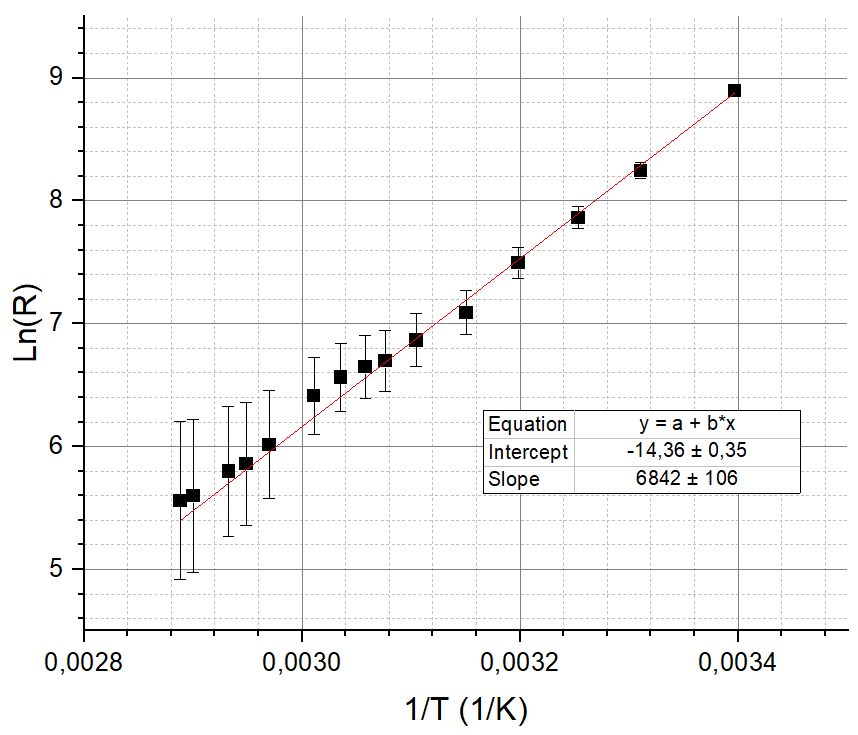
\includegraphics[width=0.9\textwidth]{gr}
\end{center}
\end{figure}


\end{document}